% 2_graalvm_truffle.tex
\begin{frame}
    \centering
    \textbf\ttfamily{\huge{Running Polyglot Programs}}
\end{frame}

\begin{frame}{Polyglot Environments}
    There are quite a few polyglot runtimes available:
    \vspace{2mm}
    \begin{itemize}
        \item GraalVM
        \vspace{2mm}
        \item Jupyter Notebooks
        \vspace{2mm}
        \item .NET Common Language Runtime
        \vspace{2mm}
        \item Et cetera
    \end{itemize}
\end{frame}

\begin{frame}{GraalVM}
    \begin{itemize}
        \item GraalVM is a high-performance runtime environment supporting multiple languages and execution modes.
        \vspace{2mm}
        \item It enhances performance through features like:
        \begin{itemize}
            \vspace{2mm}
            \item Just-in-Time (JIT) compilation.
            \vspace{2mm}
            \item Ahead-of-Time (AOT) compilation.
            \vspace{2mm}
            \item Standalone native image.
            \vspace{2mm}
            \item Polyglot API.
        \end{itemize}
    \end{itemize}
\end{frame}

\begin{frame}{GraalVM Architecture}
    \begin{figure}[h]
        \centering
        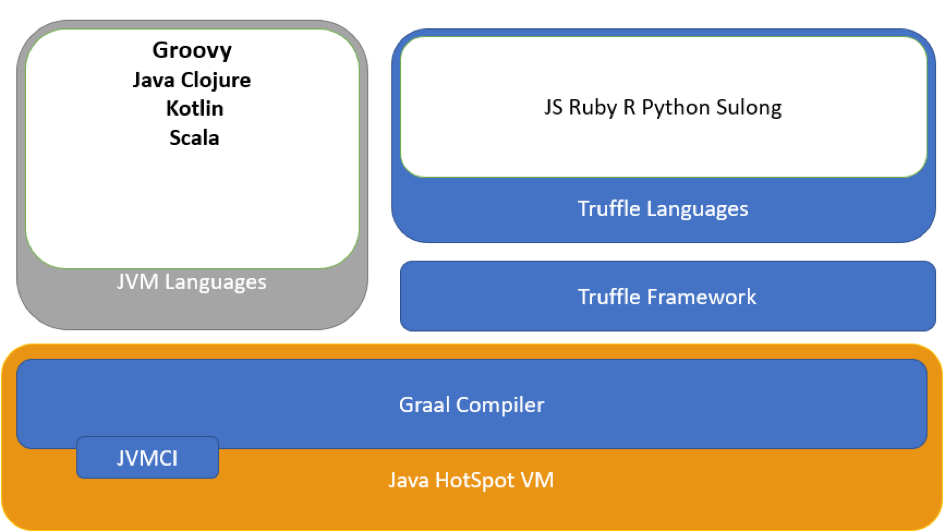
\includegraphics[width=0.7\textwidth]{images/graalvmArchitecture}
        \caption{GraalVM\tiny{(source:beyondjava.net/graalvm-plugin-replacement-to-jvm)}}
        \label{fig:graalvmArchitecture}
    \end{figure}
\end{frame}

\begin{frame}{Truffle in Nutshell}
        Language Implementation Framework:
        \begin{itemize}
            \vspace{3mm}
            \item It developers to create self-optimizing AST interpreters in Java.
        \end{itemize}
        \vspace{3mm}
        Partial Evaluator:
        \begin{itemize}
            \vspace{3mm}
            \item Uses profiling information to apply speculative optimization.
            \vspace{3mm}
            \item The interpreter get partially evaluated w.r.t the \textbf{hot} parts of the AST.
        \end{itemize}
\end{frame}

%partial eval
\begin{frame}{Partial Evaluation of User Program}
    \begin{figure}[h]
        \centering
        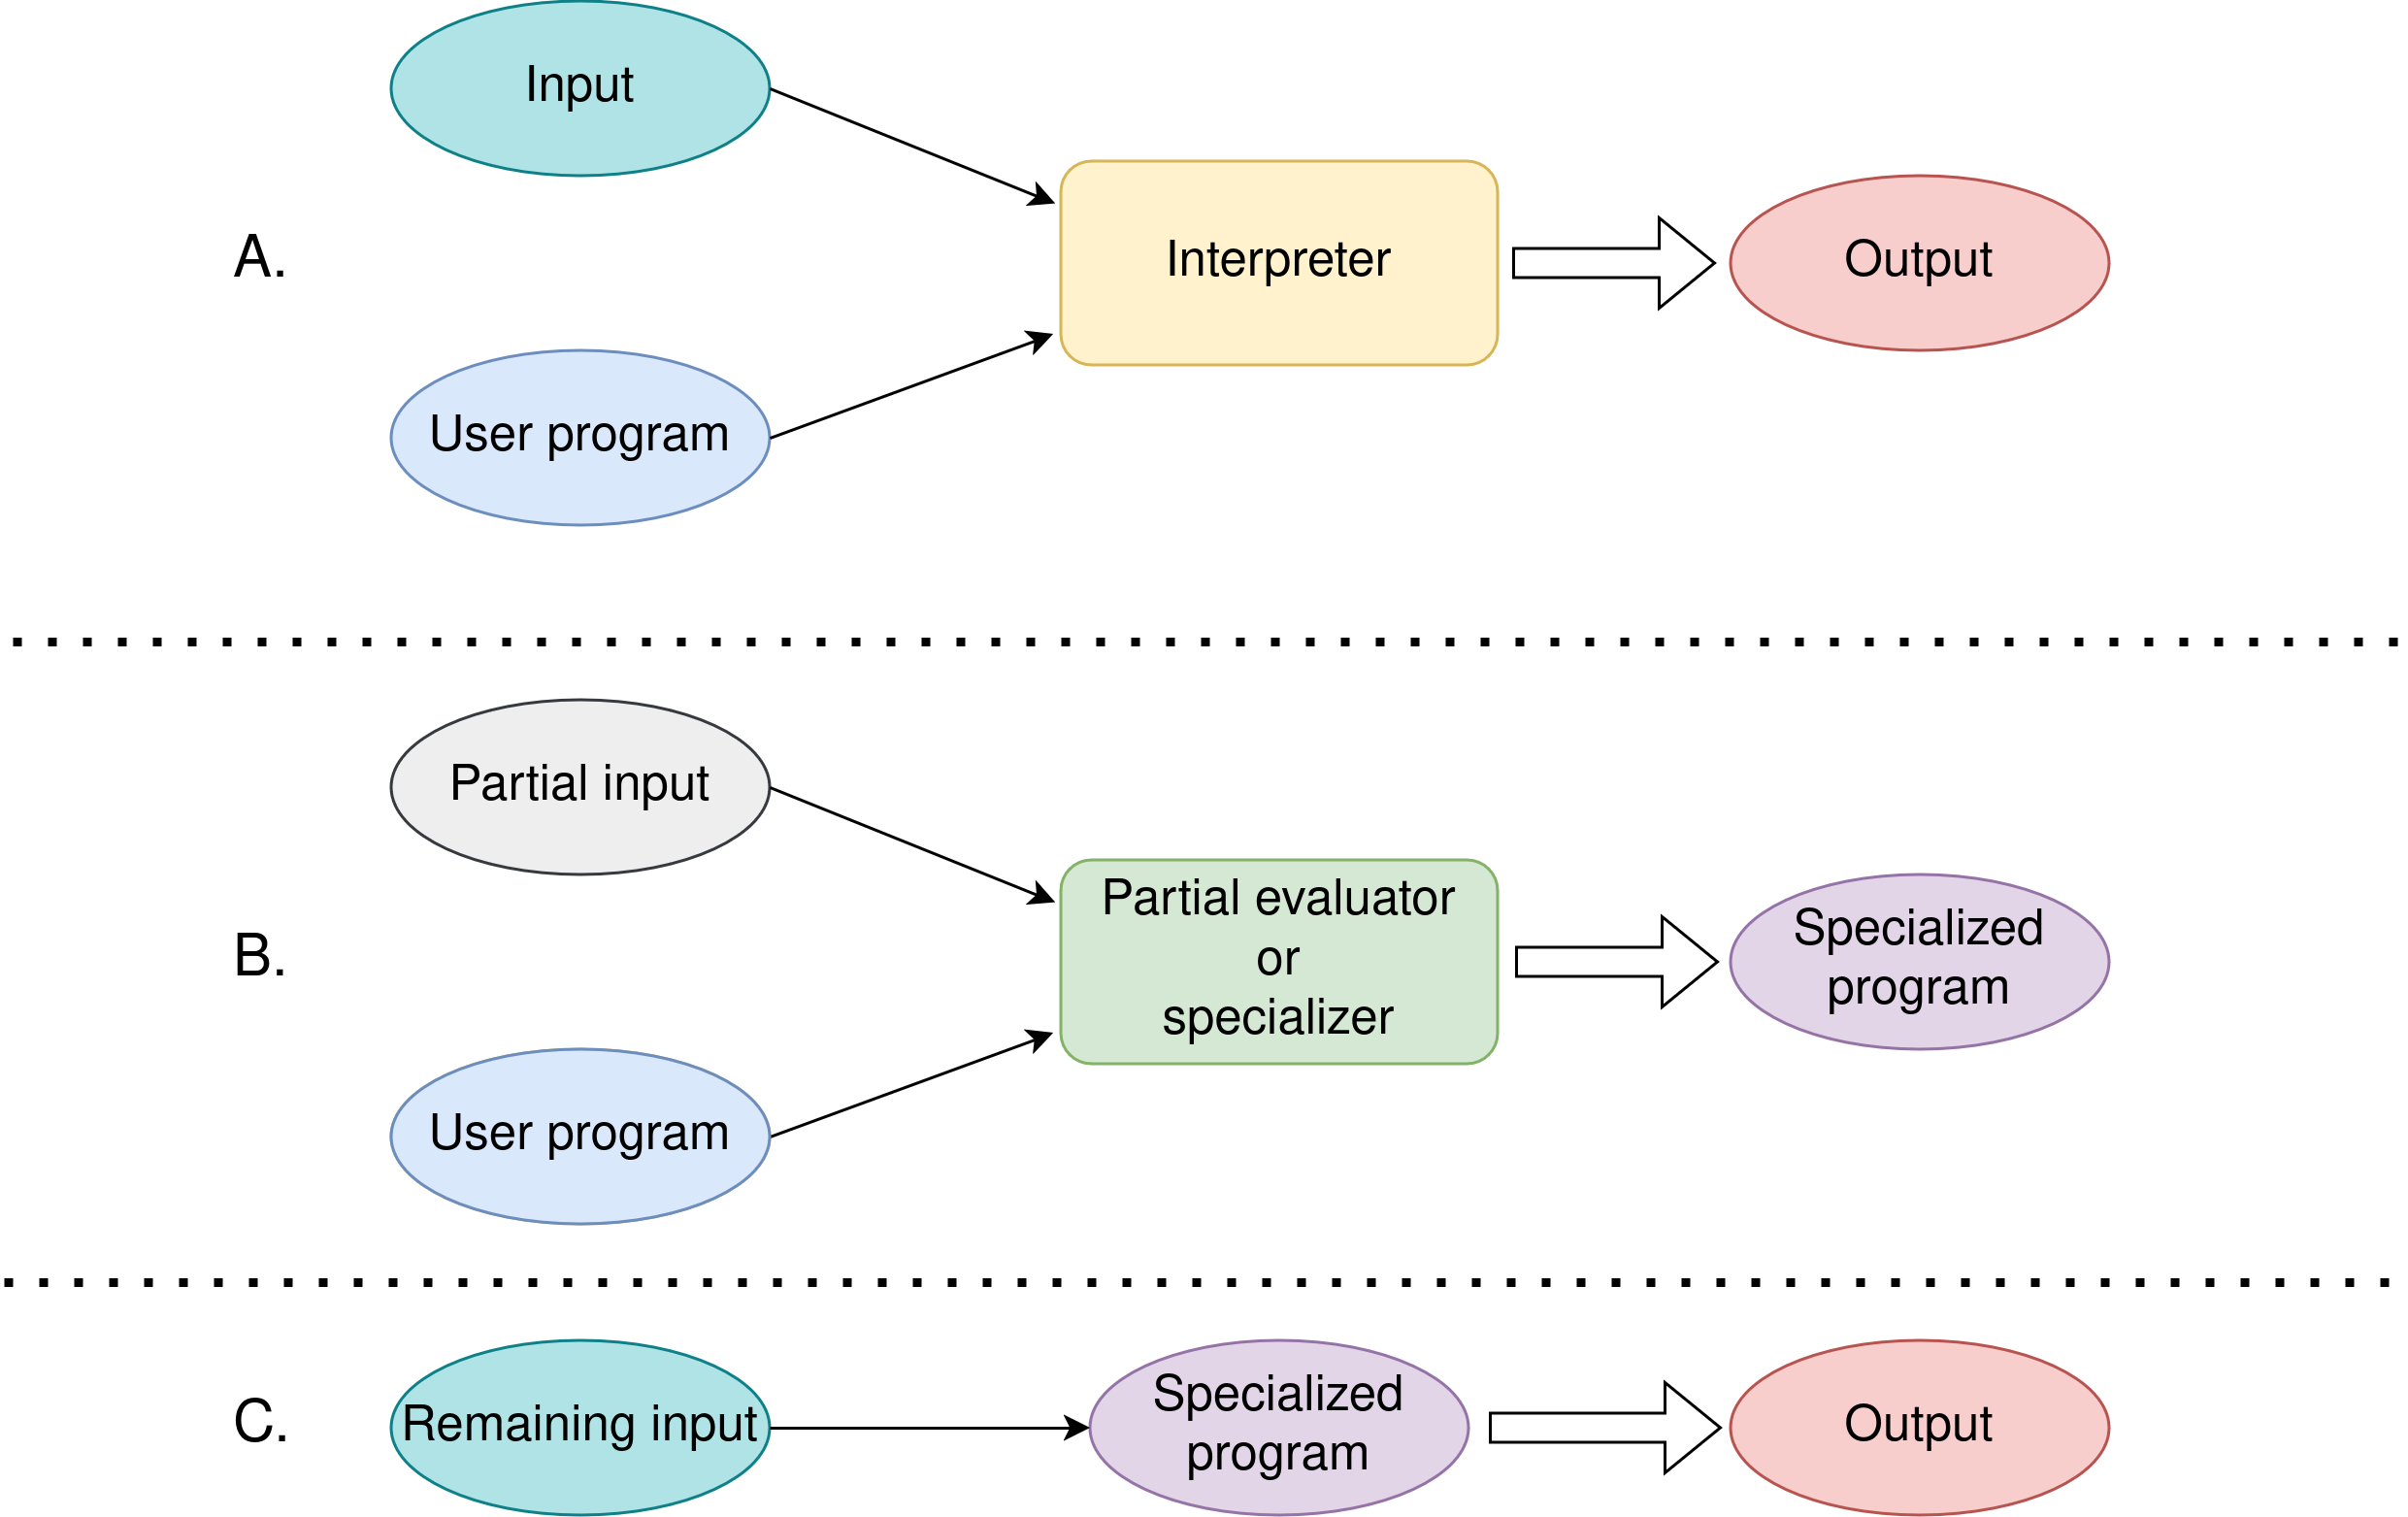
\includegraphics[width=0.6\textwidth]{images/partial-eval-of-program}
        \caption{\textbf{A)} Normal working of interpreter \textbf{B)} Specialization of program \textbf{C)} Faster code}
    \end{figure}
\end{frame}
\begin{frame}{Partial Evaluation of AST Interpreter}
    \begin{figure}[h]
        \centering
        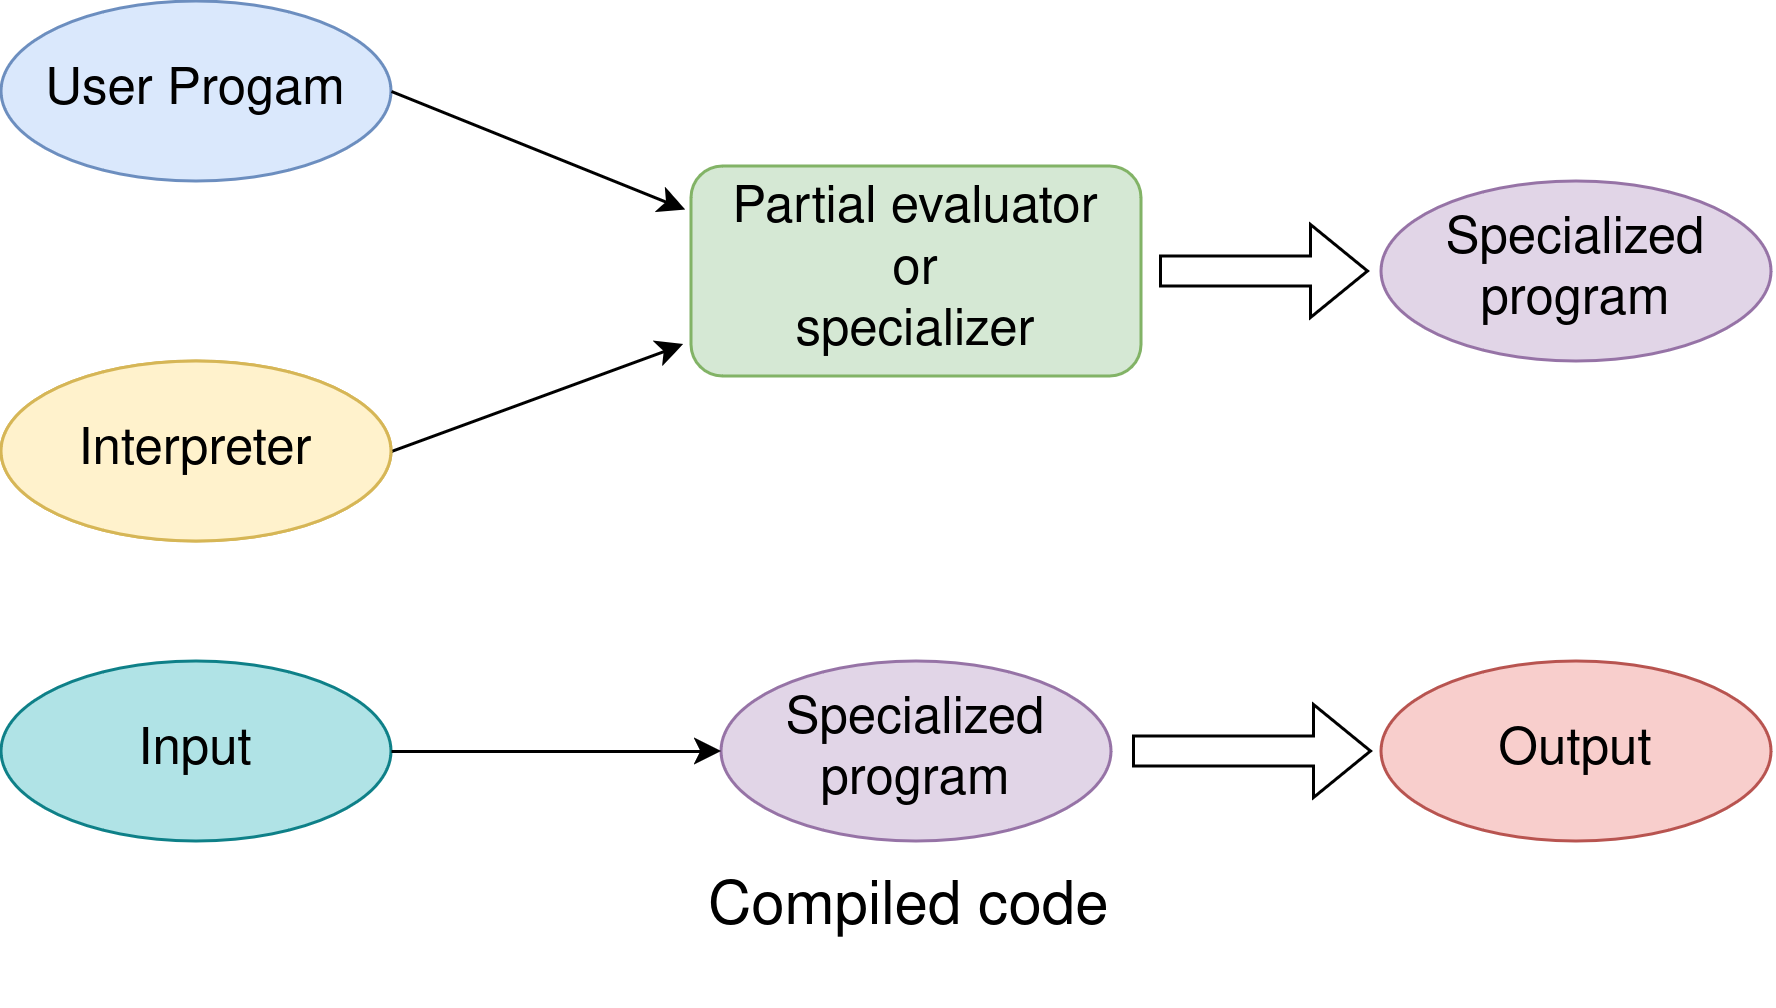
\includegraphics[width=0.6\textwidth]{images/partial-eval-of-interpreter.png}
        \caption{Partially evaluation the AST interpreter with respect to user program}
    \end{figure}
\end{frame}
